%!TEX root = Thesis_main.tex

\chapter{Controller}
\label{chapter5}

\section{Introduction and Aim of the controller}

In this chapter the core of the developed controller will be presented. The goal of our research is to solve the mobile manipulation problem of trajectory tracking for movimentation and grasping tasks. The tasks we wish to perform are in general solved decoupling the controller in order to move the mobile robot in a defined position in order to have a fixed position of the base during grasping and to reduce uncertanties in end-effector position. This approach is generally reliable since controlling indipendently the base of the robot and the arm with well known techniques allows precision and robustness. Anyway, if we want to perform the tasks in a time optimal way this approach is not suitable. The possibility to move within an enviroment during grasping operation to allow faster performance time is a goal desired not only in manipulation tasks but for many applications. Futhermore, the usage of a unique controller could allow to exploit the many degrees of redundancy to optimize other process variables such as manipulablity or obstacle avoidance capability. What we've developed, is a unique controller able to deal with the whole mobile manipulator system. The controller we developed aim to solve some of the issues presented in \ref{chapter4} by means of a Nonlinear Model Predictive Control with a novel approach to solve the online optimization problem reducing the overall computational time. The choice of MPC controller has been made for many reasons: 

\begin{itemize}
\item By means of the Reciding Horizon Principle (\ref{section_MPC}) it is possible to forecast the behaviour of the system. This approach becomes useful for obstacle avoidance and in manipulability maximization tasks.
\item It is an open framework that allows customized problems.
\item Introducing contraints allows to take into account feasibility set of the joint variable as well as control input limits.
\item Being an Optimal controller allows the minimization of customized parameters such as manipulability, control input effort etc...
\item It is generally used as a high level controller, the low level loops are in charge to track given high level command and deal with system dynamic.
\end{itemize}

In the next section will be explained the general NMPC structure for the mobile manipulation problem referring to a nonholomic vehicle and a 6 DOF's manipulator. Novel approach to reduce computational time and stability proof will be discussed later on.

\section{Problem Definition}

In this section the variables of the system and the model used for the MPC problem definition will be defined. The choice of the kinematic model instead of the dynamic one has been made for different reasons:

\begin{itemize}
\item Even if our approach allows to reduce computational time, the usage of the Dynamic model introduce further complexity in system propagation that slow down significantly the solving time.
\item Because the control action of the kinematic model is define as velocities, it's easy to implement velocity constraints.
\item Low level motor controllers are usually in charge to track velocities with higher frequency loops. This hierarchical approach is widly diffuse in controlling complex robotic systems.
\item From a user point of view, kinematic variables allows a better understanding of what's appening on the real system
\end{itemize}

\subsection{Model}

The kinematic model of the mobile manipulator is given combining \ref{dirkinMM} and \ref{base_kin_mod}. In order to do that we will define the new state variable as:
\begin{equation}
{x}(t) \in \mathbb{R}^n\ \  \textnormal{s.t.}\ \  {x}  = \left[ \begin{matrix} x \\ y \\ \theta \\ \Theta_1 \\ \Theta_2 \\ \Theta_3 \\ \Theta_4 \\ \Theta_5 \\ \Theta_6 \end{matrix} \right]\ \   \textnormal{and}\ \  {u}(t) \in \mathbb{R}^m\ \ \textnormal{s.t.}\ \ {u}=\left[ \begin{matrix} v \\ \omega \\ \dot{\Theta}_1 \\ \dot{\Theta}_2 \\ \dot{\Theta}_3 \\ \dot{\Theta}_4 \\ \dot{\Theta}_5 \\ \dot{\Theta}_6 \end{matrix} \right]
\end{equation}
By means of this variables the nonlinear kinematic model of the Nonholomic mobile manipulator can be defined as:

\begin{equation} \label{system_base}
	\dot{{x}}=f({x},{u})
\end{equation} 
Where:
\begin{equation} \label{NLsystem}
	f({x},{u}) = \left[ \begin{matrix}
	G({x}) & \textbf{0} \\ \textbf{0} & I \end{matrix} \right]
\end{equation}
and G({x}) is defined as in \ref{Gmatrix_def}:

\begin{equation}
G({x}) =  \left[
\begin{matrix}
\cos\theta & 0 \\
\sin\theta & 0 \\
0 & 1 
\end{matrix}
\right] 
\end{equation}

\subsubsection*{Notation:}
We will use the same notation of \ref{chapter3}. Briefely recalling: ${x}_{k|i}$ is the state vector at time instant $i$ propagated starting from time instant $k$, and in the same way with ${u}_{k|i}$

\subsection{NLP definition}

As done in \ref{chapter3} we will set up a minimization problem considering a quadratic cost function in the form:
\begin{equation}
J_{k}({x}_{k|i},{u}_{k|i})=\sum_{i=1}^{N}l({x}_{k|i},{u}_{k|i})
\end{equation} 
Where $l({x}_{k|i},{u}_{k|i})$ is a positive definite function dependent on the state and the control action. By including the \ref{NLsystem} and state and control feasibility boundaries the problem becomes: 

\begin{equation} \label{ourproblem_basic}
\begin{split}
		& min_{\textbf{u}}\ J({x}_{k|i},{u}_{k|i}) \\
		\textnormal{s.t.}\qquad
		&\ \ \ \ \dot{{x}}=f({x},{u}) \\
		&\ \ \ \ {x}_{k|i} \in \mathbb{X}\ \forall\ i=1,\dots,\ N  \\
		&\ \ \ \ {u}_{k|i} \in \mathbb{U}\ \forall\ i=0,\dots,\ N-1 \\
	\end{split}	
\end{equation}
where $\mathbb{X} = \lbrace {x}\in \mathbb{R}^n\ \textnormal{s.t.}\ {x}_{min}\leq x\leq x_{max} \rbrace$ is the feasible region of the state, $\mathbb{U} = \lbrace {u}\in \mathbb{R}^m\ \textnormal{s.t.}\ {u}_{min}\leq{u}\leq{u}_{max} \rbrace $ and $\textbf{u}=[\ u_{k|0},\ u_{k|1},\ \dots,\ u_{k|N-1}\ ]$.
Note that the problem has to be discretized, we will refer at $T_k$ as the discretization time, so the time between $k$ and $k+1$ as well as the time between $i$ and $i+1$.
The problem defined in \ref{ourproblem_basic} is a standard NMPC problem that can be solved using well known numerical optimization methods, where equation \ref{NLsystem} is numerically integrated to propagate the state ${x}_{k|i+1}$. Anyway the problem so defined is to find a solution $U^*\ \in\ \mathbb{R}^{mX(N-1)}\ \textnormal{s.t.}\ U^* =[{u}^*_{k|0},\ {u}^*_{k|1},\ \dots,\ {u}^*_{k|N-1}]$. Even if, according to MPC logic, only the first computed control action ${u}^*_{k|0}$ will be applied, the problem needs to be solved for all the prediction horizon. Because of that, the dimension of the problem is highly dependendt on N. Considering our case for example, we have $m=8$, so if we set $N=20$ the dimension of $U^*$ that has to be found is $8X20=160$. The dependence of the problem dimension on the optimization horizon length generate restrictions on the choice of $N$. This is due to the increase in computational time that may become too high to solve fast online applications like handling and grasping for mobile manipulators. A solution could be to bound the value of $N$ in order to keep the problem within a solvable dimension. However, some task's performance like obstacle avoidance increase as $N$ increase. For this reason we introduced a parameterized control input approach to reduce the depencende of $N$ on the solving time.

\subsection{Parameterization}

The problem defined as in \ref{ourproblem_basic} use a control action defined as picewise constant that, as explained before, brings high computational cost dependence on $N$. To solve this issue we porpose to express the control vector ${u}_{k|i}$ as a function of some parameters:
\begin{equation}\label{param_eq}
{u}_{k|i}=F(t_j){p}_k
\end{equation}
Where $\textbf{p} \in \mathbb{R}^p$ s.t. $\textbf{p}=[\ p_1,\ p_2,\ \dots,\ p_{N_p}\ ]$ and $F(t_j)$ is the matrix of the base of the new space $R^p$. The parameters  A good choice of the parameterization is made according to the phisics of the variables to be parameterized. In \cite{kelly2013mobile} a parametric optimal approach is proposed, anyway, given that the variables to be controlled are longitudinal and angular velocities, a polynomial parameterization can fit the phisical meaning requirement. A better explanation of how to choose the parameterization will be given in \ref{stabproof}.

\begin{figure}[h!]
	\centering
	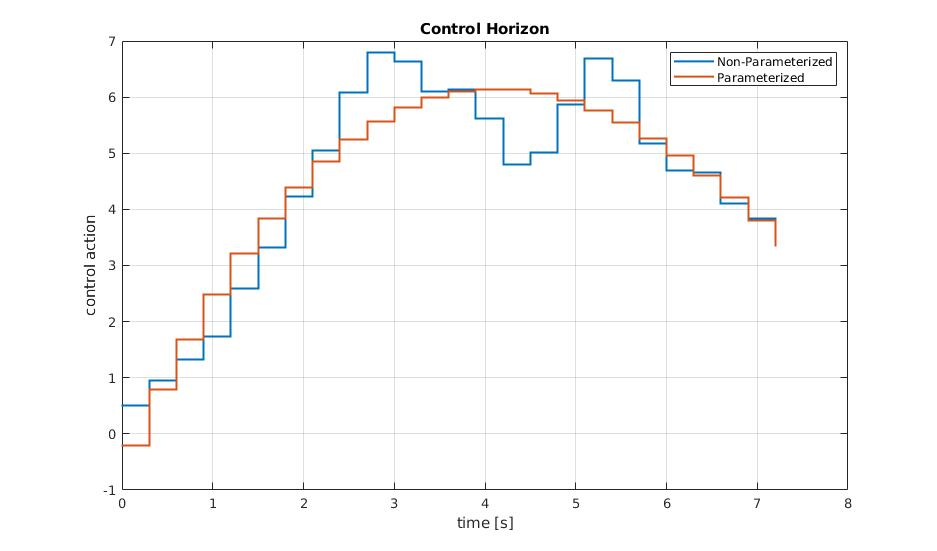
\includegraphics[scale=0.4]{param_horizon}
	\caption{Control input parameterization}
	\label{param_horizon}
\end{figure}
Considering a 3rd order Polynomial parameterization as in \ref{param_horizon} we have that each control input (i.e. each raw of the ${u}$ vector) can be expressed as a function of four parameters, for example $v=p_1i^3+p_2i^2+p_3i+p_4$.
More in general ${u}_{k|i}$ is
\begin{equation}
{u}_{k|i}=\left[ \begin{matrix}
H(i)          & \textbf{0} & \dots      & \textbf{0}  \\
\textbf{0} &     H(i)      & \dots      & \textbf{0}  \\
\vdots     & \vdots     & \ddots     & \vdots      \\
\textbf{0} & \dots      & \textbf{0} &   H(i)         \\
\end{matrix} \right] \left[ \begin{matrix} \textbf{p}_v \\ \textbf{p}_{\omega} \\ \textbf{p}_{\Theta_1} \\ \textbf{p}_{\Theta_2} \\ \vdots \\ \textbf{p}_{\Theta_6} \end{matrix} \right]
\end{equation}
Where: 
\begin{equation}
\left[ \begin{matrix} \textbf{p}_v \\ \textbf{p}_{\omega} \\ \textbf{p}_{\Theta_1} \\ \textbf{p}_{\Theta_2} \\ \vdots \\ \textbf{p}_{\Theta_6} \end{matrix} \right] = \left[ \begin{matrix} p_1 \\ p_2 \\ \vdots \\ p_{32} \end{matrix} \right]\ \ \textnormal{and }\ \ H(i)=[\ t_j^3\ \ t_j^2\ \ t_j\ \ 1\ ]
\end{equation}
Note that $t_j$  is defined as:
\begin{equation*}
	t_j=t_j(i)=T_k(i-1)\ \ \ \ \forall\ i=1,\dots,\ N-1
\end{equation*}
By applying the change of variables \ref{param_eq} into the problem formulation \ref{ourproblem_basic} we obtain:
\begin{equation} \label{ourproblem_param}
\begin{split}
		& min_{\textbf{p}_k}\ J({x}_{k|i},\textbf{p}_k) = \sum_{i=1}^{N}\tilde{l}({x}_{k|i},\textbf{p}_k) \\
		\textnormal{s.t.}\qquad
		&\ \ \ \ \dot{{x}}=\tilde{f}({x},\textbf{p},t) \\
		&\ \ \ \ {x}_{k|i} \in \mathbb{X}\ \forall\ i=1,\dots,\ N  \\
		&\ \ \ \ \textbf{p}_k\   \in \mathbb{P}\ \\
	\end{split}	
\end{equation}
Where $\mathbb{P} = \lbrace \textbf{p}\in \mathbb{R}^p\ \textnormal{s.t.}\ F(t_j(i))\textbf{p} \in \mathbb{U}\ \forall\ i = 1,\ \dots,\ N-1 \rbrace $ and $\tilde{l}$ is simply the stage cost defined as function of $\textbf{p}_k$ instead of ${u}_{k|i}$ By means of this substitution the problem has to be minimized with respect to $N_p$ parameters, that don't depend on N. In fact, using 3rd order polinomial as proposed, we have to minimize with respect to $32$ parameters, even for large prediction horizon. Implementing this approach results in a faster solution of the optimization problem, and the possibility to enlarge significantly the prediction horizon. Anyway $N$ has to be chosen properly: increasing too much the prediction horizon may result in bad performances due to overconstraining of the control action. This effect, as well as a performance comparison with respect to traditional MPC will be discussed later on.

\subsection{Increasing weights cost function definition}

Once the problem has been defined in it's general form we have to properly choose the cost function. In particular the stage cost $\tilde{l}$ has to be defined. A common choice is to use a quadratic stage cost in order to have a positive definite cost function to help in having a convex problem. Even if it's important to have a quadratic cost function for the stability of the controller, because of the nonlinearities of the system, it is still possible to find suboptimal solutions (i.e. local minima). We will define the stage cost $\tilde{l}$ as a sum of different contrubutions using increasing wheights into the optimization horizon. 

\begin{equation} \label{costfunctionh}
J({x}_{k|i},\textbf{p}_k)=\sum_{i=1}^{N}\left(\frac{i}{N}\right)^m \left[ \sum_{j=1}^{5} h_j({x}_{k|i},\textbf{p}_k) \right]
\end{equation} 
This approach allows, by means of increasing wheighted stage costs, to assess the stability of the NMPC without the imposition of terminal constraints as shown in \ref{alamir2018stability}. This aspect will be reviewed in detail later on.
The definition of the $h_j$ functions define what we want to minimize. Becauce the aim of the controller is to track the trajectory of the end-effector solving the mobile manipulation problem, we will define two stage cost ($h_1$ and $h_2$) related to the mobile manipulation problem and two more terms that will be discussed later on.  

\begin{itemize}

\item The stage cost related to the end effector position

\begin{equation}
	h_1 = [\xi_{k|i}-\xi_{{k|i}_{d}}]^T W_1[\xi_{k|i}-\xi_{{k|i}_{d}}]
\end{equation}

\begin{equation} 
 \xi_{k|i} = \left[ \begin{matrix} x_{{k|i}_{ee}} \\ y_{{k|i}_{ee}} \\ z_{{k|i}_{ee}} 
\end{matrix} \right] = \left[ \begin{matrix}
1 & 0 & 0 & 0 \\ 0 & 1 & 0 & 0 \\ 0 & 0 & 1 & 0
\end{matrix} \right]A_{{k|i}_{ee}}\left[ \begin{matrix}
0 \\ 0 \\ 0 \\ 1
\end{matrix} \right]% qui devo pensare come scrivere la posizione dell'EE in maniera compatta come funcione dello stato x, magari faccio qualche passaggio
\end{equation} 
Where $A_{{k|i}_{ee}}$ is the rototraslation matrix defined in \ref{AAAA}, $\xi_{{k|i}_{d}}$ is the desired end effector position and $W_1$ is a 3X3 weigthing matrix

\item The stage cost related to the manipulability. In order to maximize the manipulability we defined this cost as a function of to the manipulability index:
\begin{equation}
m_{k|i} =  det(\mathcal{J}_{ee}^T\mathcal{J}_{ee})
\end{equation}
Where $\mathcal{J}$ is defined as $\mathcal{J}=[\ \mathcal{J}_b(q)\ \mathcal{J}_a(q)\ ]$ like in \ref{eq:dotx_EE}. The cost is then computed as: 
\begin{equation}
	h_2 = W_2 \left( \frac{1}{m_{k|i}} \right)^2
\end{equation}
    
\item $h_3$ is the cost related to the control effort defined as: 
	\begin{equation}
	        h_3=\left[ \begin{matrix} v_{k|i-1} \\ \omega_{k|i-1} \end{matrix}\right]^T W_3 \left[ \begin{matrix} v_{k|i-1} \\ \omega_{k|i-1} \end{matrix}\right]
	 \end{equation}
This cost is particulary usefull to reduce the movement of the base given that its positioning system is less reliable than the manipulator.
\end{itemize}
We will introduce now other 2 therms that will be used instead of the previous to move the system from and towards the grasping area. Decoupling the problem with two different cost functions allows to have a faster controller during the motion of the system when it's required to have high speeds and to increase the complexity of the problem only inside a grasping area where the system moves slower to perform grasping. 
\begin{itemize}
    \item $h_4$ will be used to consider the base positioning error with respect to a given planned trajectory to reach the grasping area:
        \begin{equation}
            h_4=[q_b-{q_b}_d]^T W_4 [q_b-{q_b}_d]
        \end{equation}
        Where ${q_b}_d$ is the desired state of the base of the MM at time instant i. \\
    \item $h_5$ will be used to control the arm in joint space, so to track a desired Joint position ${q_m}_d$:
    \begin{equation}
       h_4=[q_m-{q_m}_d]^T W_5 [q_m-{q_m}_d]
    \end{equation}
     
    This therm is particularly useful to simplify the problem during the motion of the base because it allows to directly compute the error without passing through the forward kinematics.
\end{itemize}


% poi appunto parliamo di h2 che sarebbe la parte legata alla manipolabilità e diciamo bene che come detto nel cap 4?? la manipolabilità si può trattare in diversi modi e noi ne abbiamo scelto uno

%poi si può dire a questo punto che esistono altri termini che volendo si possono aggiungere per rendere più completo il controllore e semplificare la soluzione per esempio

% qui passo a parlare di h3 che sarebbe l'errore sulla base e spieghiamo che poi dal punto di vista del codice questa parte non è findamentale nel senso che la traiettoria sarebbe disponibile ma non la usiamo perchè vogliamo che sia il controllore a risolvere il problema di mobile manipulation

% eventualmente ci mettiamo h4 (cambiare numeri) e diciamo che ci serve solo per semplificare il tenere fermo il manipolatore in movimentazione per il motivo del costo etc....

%così è definita la funcione di costo 

%\\ x_{ee} \\ y_{ee} \\ z_{ee} \\ \phi_{1_{ee}} \\ \phi_{2_{ee}} \\ \phi_{3_{ee}}

\section{Stability Proof}\label{stabproof}

Once the NMPC problem has been formulated and that the recursive feasibility of the problem has been easily investigated in \ref{chapter3}, its stability has to be assessed. 
The proof is very similar to what done in \cite{alamir2018stability} with few modifications. We will consider now, for the stability proof, the tracking problem in a differnt form to treat the tracking problem as a zero-reference tracking problem. In order to do that we will consider:
\begin{equation*}
    e_k=x_k-{x_k}_d
\end{equation*}
and so the discretizing the state equation \ref{system_base} we have:
\begin{equation}\label{sys_eq_con_e}
    e_{k|i+1}=\hat{f}(e_{k|i},p_k,{x_{k|i}}_d,{x_{k|i+1}}_d)
\end{equation}
In this way the problem is moved to track zero error reference and becomes: 
\begin{equation} \label{ourproblem_stab}
\begin{split}
		& min_{{p}_k}\ J({e}_{k|i},{p}_k) =\sum_{i=1}^{N}\hat{l}(e_{k|i},{p}_{k}) \\
		\textnormal{s.t.}\qquad
		&\ \ \ \ e_{k|i+1}=\hat{f}(e_{k|i},p_k) \\
		&\ \ \ \ e_{k|i} \in \mathbb{E}\ \forall\ i=1,\dots,\ N  \\
		&\ \ \ \ {p}_k\   \in \mathbb{P}\ \\
	\end{split}	
\end{equation}
where $\mathbb{E} = \lbrace {e}\in \mathbb{R}^n\ \textnormal{s.t.}\ {e}_{min}\leq e\leq e_{max} \rbrace$ is the feasible region of the state error. Note that, for simplicity of notation, the system equation in \ref{sys_eq_con_e} has been expressed as a function of the previous state and the parameters only, given that the desired states are known.
Now, following the \cite{alamir2018stability} we need to introduce some assumptions in order to assess stability of the controller. The proof will consider some modification of what done in \cite{alamir2018stability} to consider the parametrization of the control input. 


\paragraph{Assumption 1} The maps of $\hat{f}$ and $\hat{l}$ are continuous and $\hat{l}$ is a positive definite function. 

\paragraph{Assumption 2} We will introduce also a reachibility requirement, so that $\exists \textnormal{ a set } \mathbb{E}_N$ so that $\forall e \in \mathbb{E}_N $ the set:
\begin{equation*}
	\mathbb{P}_{e \to 0}:=\lbrace \ p \in \mathbb{P}\ s.t.\ e_N^p(e)=0\ \rbrace
\end{equation*} exsist and is not empty.

\paragraph{Assumption 3} Is a local control invariance property assumend in the neighberhood of the origin, i.e. there exsist a $\bar{\rho} > 0$ such that:
\begin{equation}
	\begin{split}
		\forall \rho &\leq \bar{\rho}, \forall e \in B_{\it{l}}(\rho),\exists\ p^+\textnormal{s.t.} \\
		&\hat{l}(\hat{f}(e,p))-\hat{l}(e) \leq -q(e) \\
		\label{ass3}
	\end{split}
\end{equation}
for some positive definite function $q$ that satisfy:
\begin{equation}
	q(e) \ge \gamma l(e)
	\label{ass3} 
\end{equation}
for some $\gamma \geq 0$ and $\forall x \in \mathbb{X}$.
Where $B_{\it{l}} \subset \mathbb{R}^n$ is the $\rho-$level set of $l$, defined as $B_{\it{l}} := \lbrace\ e \in \mathbb{R}^n\ |\ l(e) \leq \rho \rbrace$.

\paragraph{Assumption 4} We will require an extended control input parameterization vector $p:=[p_1,\ p_2,\ \dots,\ p_{N_p},\ k^*]$ such that: 
\begin{equation*}
\begin{split}
    u_{k|j}(p_k)=
        \begin{cases}
            F(j){p_k}\ \ \ \ \   &\textnormal{if } j<k^* \\
            \Bar{u}=argmin_u l(\hat{f}(e_{k|N},u_k))\ \ &\textnormal{if } j\ge k^*
        \end{cases}
    \end{split}
\end{equation*} 
Then given the optimal solution at time instant $k$ defined as $p_k^*=[\ p_{k_1}^*,\ p_{k_2}^*,\  \dots,\  p_{k_{N-1}}^*\ ]$ that corresponds to $  \textbf{u}_k^*=[\ u_{k|0}^*,\ u_{k|1}^*,\  \dots,\  u_{k|{N-1}}^*\ ]$ it is possible to obtain the parameters $\tilde{p}_{k+1}$ such that the correspondent control input is $  \textbf{u}_{k+1}^*=[\ u_{k|1}^*,\ u_{k|2}^*,\  \dots,\  u_{k|{N-1}},\ \Bar{u}^* \ ]$.
That means to require that the parameterization function $F$ is translatable (see \ref{param_translatability}). \\
\begin{figure}[h!]
	\centering
	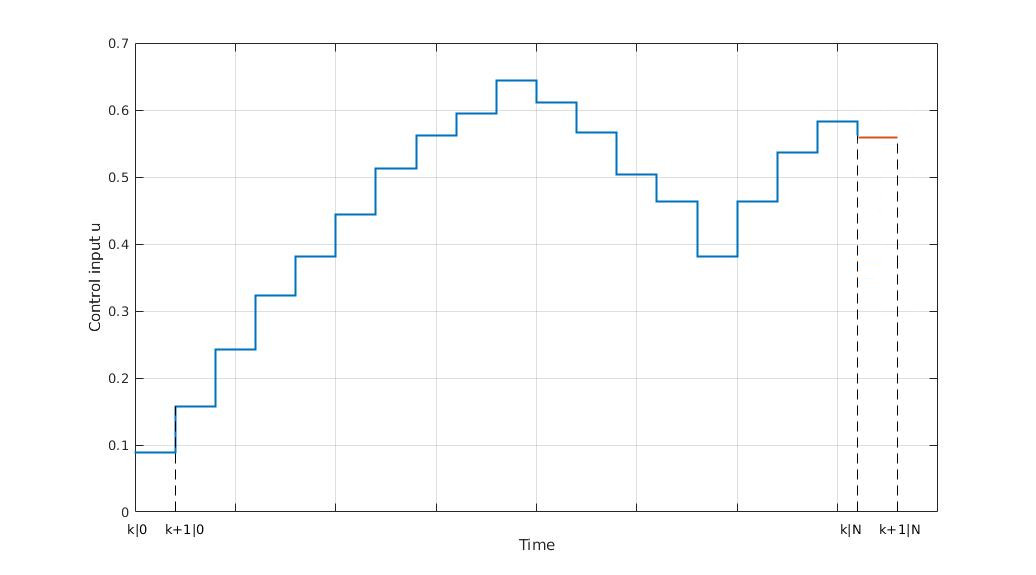
\includegraphics[scale=0.4]{IMMAGINI/trans_u}
	\caption{Translatability of the $F$ function}
	\label{param_translatability}
\end{figure}

\paragraph{Lemma 1} Under Assumption 1, $\forall e \in \mathbb{E}^N$, one as:
\begin{equation}
	l(e_N^{p*}) \leq \eta\ c^m\ \ \  \textnormal{where    } c:=\frac{N-1}{N} < 1
 	\label{lemma1}
\end{equation}
for some bounded $\eta < 0$. The proof of Lemma 1 is given in \cite{alamir2018stability}. \\



%%%%%%%%%%

In order to assess stability is required that the cost function $J({e}_{k|i},{p}_k)$ is a Lyapunov function as explained in \ref{chapter3}. So, considering the cost function related to $\tilde{p}_{k+1}$ is:
\begin{equation*}
    J({e}_{k+1|i},\tilde{p}_{k+1})=\sum_{i=1}^{N-1}\left(\frac{i}{N}\right)^m h({e}_{k|i},\tilde{p}_{k+1})+h(\hat{f}(e_{k|N},u_k))
\end{equation*}
Now considering $j=i+1$ and to simplify notation $h(e_{k|j})^*=h({e}_{k|i},p_{k}^*)$ follows: 
\begin{equation*}
    J({e}_{k+1|i},\tilde{p}_{k+1})=\sum_{j=2}^{N}\left(\frac{j-1}{N}\right)^m h(e_{k|j})^*+h(\tilde{f}(e_{k|N},u_k))
\end{equation*}
Now rearranging the terms: 
\begin{equation*}
    \begin{split}
        J({e}_{k+1|i},\tilde{p}_{k+1})=&\sum_{j=2}^{N}\left[\left(\frac{j-1}{N}\right)^m-1\right]\left(\frac{j}{N}\right)^m h(e_{k|j})^*+ \\
        &+\sum_{j=2}^{N}\left(\frac{j}{N}\right)^m h(e_{k|j})^* + h(\hat{f}(e_{k|N},u_k))
    \end{split}
\end{equation*}
Note that 
\begin{equation*}
	\sum_{j=2}^{N}\left(\frac{j}{N}\right)^m h(e_{k|j})^*=J({e}_{k|i},p_{k}^*)-\frac{1}{N^m}h(e_{k|1})^*
\end{equation*}
we get:
\begin{equation*}
    \begin{split}
        J({e}_{k+1|i},\tilde{p}_{k+1})=&J({e}_{k|i},p_{k}^*)-\frac{1}{N^m}h(e_{k|1})^*+ \\ 
        &-\sum_{j=2}^{N}\left[1-\left(\frac{j-1}{N}\right)^m\right]\left(\frac{j}{N}\right)^m h(e_{k|j})^*+ h(\hat{f}(e_{k|N},u_k))
    \end{split}
\end{equation*}
And because $\forall j \in \lbrace2,\ \dots,\ N\rbrace$ holds that: 
$\left[ 1-\left(\frac{j-1}{N}\right)^m \right]\ge\left[ 1-\left(\frac{N-1}{N}\right)^m \right]= \phi(m)$. We can then say that: 
\begin{equation}\label{dim1}
    \begin{split}
        J({e}_{k|i},\tilde{p}_{k+1})\le &J({e}_{k|i},p_{k}^*) - \frac{1}{N^m}h(e_{k|1})^*+ \\ 
        &-\phi(m)\sum_{j=2}^{N}\left(\frac{j}{N}\right)^m h(e_{k|j})^*+ h(\hat{f}(e_{k|N},u_k))
    \end{split}
\end{equation}

Now according to Lemma 1, $e_N^{p*} \in B_l(\eta c^m)$ and together with Assumption 2 implies that for m sufficiently high, is it possible to say:

\begin{equation}
\eta c^m \leq \bar{\rho}
\end{equation}

where $\bar{\rho}$ is the positive real called in Assumption 3.
This means that \ref{ass3} holds for $e_N^{p*}$ and we can say that:
\begin{equation*}
    h(\tilde{f}(e_{k|N},u_k)) \le h(e_{k|N})^*-q(e_{k|N},p_k^*)
\end{equation*}
By applying this relation on the \ref{dim1} we obtain: 
\begin{equation*}
    \begin{split}
        J({e}_{k|i},\tilde{p}_{k+1})\le &J({e}_{k|i},p_{k}^*) - \frac{1}{N^m}h(e_{k|1})^*+ \\ 
        &-\phi(m)\sum_{j=2}^{N}\left(\frac{j}{N}\right)^m h(e_{k|j})^*+ h(e_{k|N})^*-q(e_{k|N},p_k^*)
    \end{split}
\end{equation*}
Then using the \ref{ass3}:
\begin{equation*}
    \begin{split}
        J({e}_{k|i},\tilde{p}_{k+1})&\le J({e}_{k|i},p_{k}^*) - \frac{1}{N^m}h(e_{k|1})^*+ \\ 
            &-(\phi(m)-1+\gamma)\ h(e_{k|N})^*
    \end{split}
\end{equation*}
Noting that $\phi(m) \rightarrow 1$ for $m \rightarrow \infty$, for sufficiently high values of m, $J$ is a Lyapunov function. It follows that the closed loop system is asymptotically stable in $e=0$.


%vedi slides

\section{Constraints}

Constraints will be introduced in order to properly define the problem taking into account feasibiity configurations, maximum velocity and acceleration as well as to avoid self collision of the system. In particular the constraints definition has been divided into: 

\subsubsection*{Joint position constraints}
	To limit the configurations of the robot into feasible sets and to avoid the arm to self collide there are different approaches. We decided to limit the possible positions of the joints of the arm into feasible ranges. This means to generate a set:
	\begin{equation}
		\mathbb{R}^{q_m}:=q_m \in \mathbb{R}^{q_m}\ \ s.t.\ \  {q_m}_{min}\ \leq\ q_m\ \leq\ {q_m}_{max} 
	\end{equation}
	To apply this constraint into the MPC problem defined in \ref{ourproblem_param} is straigthforward given that $\mathbb{R}^{q_m}$ is a subset of $\mathbb{X}$
\subsubsection*{Base position constraints}
	Contrary to the manipulator, self collision of the base of the system is not possible and the joint $q_b$ could remain unconstrained. Anyway, the $x$ and $y$ coordinates of the base have been limited to define a region of operation for the Mobile Manipulator, see as example figure \ref{xy_limits}. This constraint is particulary usefull performing experiments deining a map of the sorrounding enviroment. As before: 
	\begin{equation}
		\mathbb{R}^{q_b}:=q_b \in \mathbb{R}^{q_b}\ \ s.t.\ \  {q_b}_{min}\ \leq\ q_b\ \leq\ {q_b}_{max} 
	\end{equation}

	\begin{figure}[h!]
	\centering
	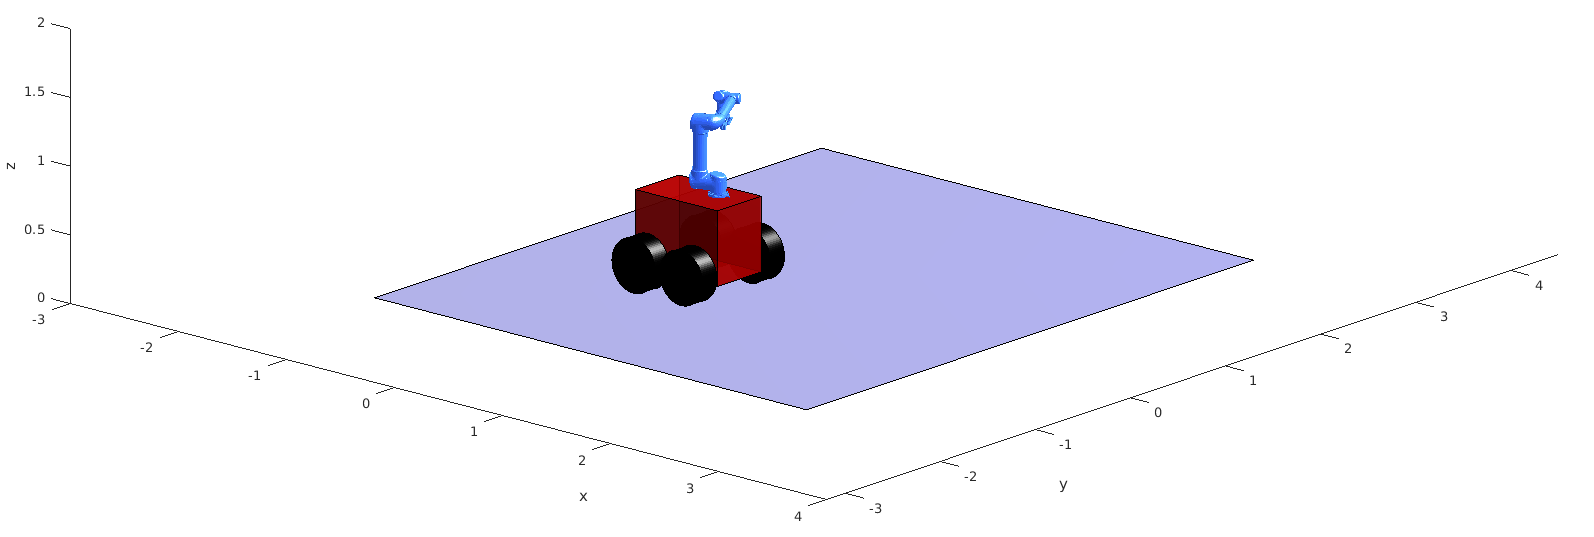
\includegraphics[scale=0.25]{IMMAGINI/xy_limits.png}
	\caption{Base $x-y$ limits}
	\label{xy_limits}
	\end{figure}

	Base and joints position constraints can be written in a compact form and for the entire prediction horizon redefining: 

	\begin{equation}
	\mathbb{X}:= x \in \mathbb{R}^{n}\ \ s.t.\ \  {x}_{min}\ \leq\ x\ \leq\ {x}_{max}
	\end{equation}

\subsubsection*{Velocity constraints}
	To take into account the maximum velcities allowed by the system, the control actions have been limited into minimum and maximum velocities according to manufacturer data in particular $\mathbb{R}^m$ have been redefined as:

	\begin{equation*}
	\mathbb{R}^m:=\ {u}_{k|i} \in \mathbb{R}^m\ \ \textnormal{s.t.}\ \ u_{min}\leq{u_{k|i}}\leq u_{max}\ \ \forall\ \  i=0,\ \dots,\ N-1
	\label{vel_constr}
	\end{equation*}
	According to the parameterization chosen, the constraint has to be defined in parametric form, i.e. we have to map $\mathbb{R}^m$ in $\mathbb{P}$. The constraint to be included in the problem \ref{ourproblem_param} requires that:
	\begin{equation*}
		\mathbb{P}:=p_k \in \mathbb{P} \textnormal{  s.t. \ref{vel_constr} is satisfied}
	\end{equation*}

	Numerical values will be given in the next section.
\subsubsection*{Acceleration constraints}
	Given that any real system is not capable to perform infinte accelerations, a constraint to limit the computed velocity control input has to be defined. In particular, given that the controller compute control actions with a frequency $f_c=\frac{1}{T_j}$, the acceleration constraint is in the form:

	\begin{equation}
		\begin{split}
			u_{k|0} &\leq u_{k-1|N-1} + a_{max} T_j\ \ \textnormal{and}\\
			u_{k|i+1} &\leq u_{k|i} + a_{max} T_j\ \  \forall\ i=0,\dots,N-1
		\end{split}	
	\end{equation}  

	Where $a_{max}$ is the vector of the maximum allowable acceleration. Numerical values will be given in the next section. 

\subsubsection*{Self collision avoidance}
	To avoid self collosion of the system (i.e. the arm with the base), an approach similar to the one in \cite{sandberg1988collision} has been used. In particular spheres to encompass the base and the last joints have been defined ans in figure \ref{spheres_3d}.
	\begin{figure}[h!]
	\centering
	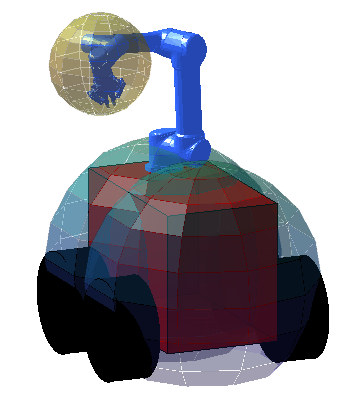
\includegraphics[scale=0.4]{IMMAGINI/spheres_3d.png}
	\caption{Spheres for self collision avoidance}
	\label{spheres_3d}	
	\end{figure}
	Formally the self collision avoidance constraint has been defined requiring that: 
	\begin{equation}
	\begin{split} 
		&\sqrt{({C_0}_x-{C_1}_x)^2+({C_0}_y-{C_1}_y)^2+({C_0}_z-{C_1}_z)^2} + r_1 +r_0 \geq 0 \\
		&\ \ \ \ \textnormal{and} \\
		&\sqrt{({C_0}_x-{C_2}_x)^2+({C_0}_y-{C_2}_y)^2+({C_0}_z-{C_2}_z)^2} + r_2 +r_0 \geq 0 \\
		&\ \ \ \ \textnormal{whith} \\
		\ \ \ \ \ \ & \ \ \ \ \ \ \  \ \ \ \ \ \left[ \begin{matrix}
		{C_0}_x \\ {C_0}_y \\ {C_0}_z
		\end{matrix} \right]=\left[ \begin{matrix}
		1 & 0 & 0 & 0 \\ 0 & 1 & 0 & 0 \\ 0 & 0 & 1 & 0
		\end{matrix} \right]A_{{k|i}_{sp}}\left[ \begin{matrix}
		0 \\ 0 \\ 0 \\ 1\end{matrix} \right]
	\end{split}
	\label{spheres_const}
	\end{equation}
	Where $A_{{k|i}_{sp}}$ is the rototranslation matrix that defines the center of the sphere encompassing the last links of the arm at time instant $i$ defined as done for the end effector in \ref{AAAA_man}. Note that, because of that, ${C_0}$ is defined in the relative reference frame of the manipulator. ${C_1}$ and ${C_2}$, defined in their components $x$, $y$ and $z$, are the centers of the two spheres for the base defined in the reference frame of the arm that are, indeed, fixed. Their radius are defined as $r_1$ and $r_2$. This constraints definition introduces a nonlinear equation that has to be satiflied in the solution of the \ref{ourproblem_param}. \\

Summarizing, the presented constraints redefines the problem as:

\begin{equation} \label{ourproblem_param}
	\begin{split}
			& min_{\textbf{p}_k}\ J({x}_{k|i},\textbf{p}_k) = \sum_{i=1}^{N}\tilde{l}({x}_{k|i},\textbf{p}_k) \\
			\textnormal{s.t.}\qquad
			&\ \ \ \ \dot{{x}}=\tilde{f}({x},\textbf{p},t) \\
			&\ \ \ \ {x}_{min}\ \leq\ x_{k|i}\ \leq\ {x}_{max}\  \forall\ i=1,\dots,\ N  \\
			&\ \ \ \ 0 \leq g^{sc}_{k|i}(x)\ \ \forall\ i=1,\dots,\ N \\
			&\ \ \ \ \textbf{p}_k\   \in \mathbb{P}\ \\
	\end{split}	
\end{equation}
where $g^{sc}_{k|i}(x)$ i the function that defines the spheres constraints as in \ref{spheres_const}

